\begin{savequote}[75mm]
Strike hot iron and call forth sparks; strike a man and call forth fury; to shape man or metal to thy will, thou must
strike with force.
\qauthor{Collected Sermons of Carras, Thief by Looking Glass Studios}
\end{savequote}

\chapter{Eksperyment numeryczny}
\section{Metodyka}
\label{sec:metodyka}
Badania zaprezentowane w niniejszej pracy bazują na szeregu eksperymentów
numerycznych wykonanych z pomocą autorskiego kodu płynowego \textsc{PIERNIK} tworzonego
od 2006 roku w Centrum Astronomii UMK.  Algorytmy numeryczne kodu
\textsc{PIERNIK}
opierają się na zachowawczym schemacie płynowym typu ,,Relaxing
TVD''~\cite{jin-xin-95} w połączeniu z~dzielonym, kierunkowym całkowaniem
przestrzennym i~czasowym przy użyciu algorytmu Runge-Kutta drugiego
rzędu~\cite{2003PASP..115..303T,2003ApJS..149..447P}. Konstrukcja kodu umożliwia
modelowanie wieloskładnikowego ośrodka np. płynu neutralnego i~płynu
bezciśnieniowego (pył) z uwzględnieniem oddziaływań
międzypłynowych~\cite{piernik1,piernik2}. \textsc{PIERNIK} wyposażony jest w
wielosiatkowy algorytm przeznaczony do wyznaczania przybliżonych rozwiązań
równań różniczkowych różnych typów, a w szczególności
solwer multigridowy pozwalający efektywnie rozwiązywać paraboliczne
i~eli\-pty\-czne równania różniczkowe, w~tym równanie Poissona opisujące
samograwitację pyłu~\citep{HG00}. Algorytm wielosiatkowy wspierany jest
algorytmem multipolowym pozwalającym na szybkie określenie warunków brzegowych
dla potencjału grawitacyjnego~\citep{J77} oraz algorytmem opartym na metodzie
sprzężonych gradientów~\cite{pcg}. Dzięki implementacji schematu płynowego
postaci zachowującej moment pędu w cylindrycznej siatce
współrzędnych~\cite{M07,SO10} możliwe są  precyzyjne  symulacje dysków
astrofizycznych. Implementacja szybkiego algorytmu eulerowskiego~\footnote{ang.
\emph{Fast Advection in Rotating Gaseous Objects -- FARGO}}~\citep{M00} w~ujęciu
wielopłynowym umożliwia znaczące przyspieszenie  symulacji wysokiej
rozdzielczości w trzech wymiarach.  Ponadto \textsc{PIERNIK} korzysta z~algorytmu typu
\emph{Constraint Transport}~\cite{EH88} zapewniającego spełnienie warunku
bezźródłowości pola magnetycznego, a także możliwość wykonywania symulacji przy
użyciu siatek adaptywnych~\footnote{ang.  \emph{Adaptive Mesh Refinement --
AMR}}. Kod został zrównoleglony przy użyciu protokołu MPI i wykazuje dobrą silną
jak i bardzo dobrą słabą skalowalność w zakresie do $10^4$ rdzeni
obliczeniowych.
%
\par Obliczenia opisywane w~tej pracy zostały przeprowadzone z~wykorzystaniem:

\begin{itemize}
   \item infrastruktury PL-Grid, w~szczególności klastrów
      komputerowych Galera+ (Trójmiejska Akademicka Sieć Komputerowa), Hydra
      (Interdyscyplinarne Centrum Modelowania Matematycznego i Komputerowego),
      Zeus (Akademickie Centrum Komputerowe CYFRONET), Inula (Poznańskie Centrum
      Superkomputerowo Sieciowe) w~ramach grantu \emph{plggpiernik},

   \item klastrów PRACE, w~szczególności klastrów komputerowych
      Cartesius (SurfSara), Fionn (Irish Centre for High-end Computing) w~ramach grantu \emph{PIERNIK-SI} w
      projekcie Distributed European Computing Initiative (DECI-11).
\end{itemize}
Sumaryczne zużycie wyniosło kilka milionów CPUh.


%We conduct numerical simulations with the aid of a
%parallel MHD code PIERNIK using the cylindrical coordinate system. 


\subsection{Podstawowe równania}
W dalszych rozważaniach założymy, że opis dynamiki gazowo-pyłowego dysku
okołogwiazdowego może być oparty na układzie równań opisujących dwa oddziałujące
dynamicznie płyny - gaz w przybliżeniu izotermicznym oraz  pył traktowany jako
płyn bezciśnieniowy. Równania hydrodynamiki przyjmują dla takiego modelu
następującą postać:
%
% CONSERVATIVE FORM
\begin{align}
   \partial_t \rho_g &+ \nabla\cdot\left(\rho_g\mathbf{u}\right) = 0,\label{eq1}\\
   \partial_t \rho_d &+ \nabla\cdot\left(\rho_d\mathbf{w}\right) = 0,\label{eq2}\\
\partial_t \left(\rho_g\mathbf{u}\right) &+
   \nabla\cdot(\mathbf{u}\otimes(\rho_g\mathbf{u})+P) \notag\\
 &= -\rho_g\left(\nabla\Phi +
\frac{\rho_d}{\tau_f\rho_g}(\mathbf{u}-\mathbf{w})\right),\label{eq3}\\
\partial_t \left(\rho_d\mathbf{w}\right) &+
\nabla\cdot(\mathbf{w}\otimes(\rho_d\mathbf{w})) \notag\\
 &= -\rho_d\left(\nabla\Phi + \frac{1}{\tau_f}(\mathbf{w}-\mathbf{u})\right)
\label{eq4}.
\end{align}
% NON-CONSERVATIVE FORM
%\begin{align}
%\partial_t \rho_g &+ \nabla\cdot\left(\rho_g\mathbf{u}\right) = 0,\\
%\partial_t \rho_d &+ \nabla\cdot\left(\rho_d\mathbf{w}\right) = 0,\\
%\partial_t \mathbf{u} &+ \left(\mathbf{u}\cdot\nabla\right)\mathbf{u} = 
% -\nabla\Phi + \frac{\rho_d}{\tau_f\rho_g}(\mathbf{w}-\mathbf{u})
% -c_s^2\nabla\ln\rho_g,\label{eq3} \\
%\partial_t \mathbf{w} &+ \left(\mathbf{w}\cdot\nabla\right)\mathbf{w} = 
% -\nabla\Phi - \frac{1}{\tau_f}(\mathbf{w}-\mathbf{u}),\label{eq4}
%\end{align}

\noindent gdzie $\rho_g$, $\rho_d$ to odpowiednio gęstości gazu i~pyłu,
$\mathbf{u}$, $\mathbf{w}$ ich prędkości, $P$ to ciśnienie gazu, $\tau_f$ jest
skalą czasową tarcia~\footnote{ang. friction time}~\mref{eq:tauf}, a $\Phi$ to
potencjał grawitacyjny.

\par Ze względu na specyfikę zagadnienia badanego w~niniejszej pracy
najwygodniejszym układem współrzędnych jest układ cylindryczny. W~kodzie
\textsc{PIERNIK}
równania mechaniki płynów w geometrii cylindrycznej wyrażone są w postaci
zachowującej moment pędu~\cite{M07,SO10}, która wprowadza tylko jeden, dodatkowy
wyraz źródłowy do równań ruchu~\mref{eq3} - \mref{eq4}: odpowiednio
$\left((\rho_g u_\phi + P) / R\right)\mathbf{\hat{R}}$ oraz $(\rho_d w_\phi / R)
\mathbf{\hat{R}}$.
%
\par Przyspieszenie będące skutkiem wzajemnego oddziaływania pyłu i gazu
przyjmuje postać $\rho_d/\tau_f\rho_g(\mathbf{u}-\mathbf{w})$
i~$1/\tau_f(\mathbf{w}-\mathbf{u})$ odpowiednio dla równań \mref{eq3}
i~\mref{eq4} w~zależności od tego jak zostanie potraktowane, może prowadzić do
znacznego skrócenia kroku czasowego. Z tego względu zdecydowano o implementacji
pół niejawnego schematu modyfikującego bezpośrednio prędkości gazu i~pyłu,
opisanego w pracy~\cite{TB09}.

%W~ramach pracy skupiono się na dyskach rozciągających się relatywnie dużych
%promienii tj. 2~AU. Zakładając, za pracą~\cite{CD93}, że przejście do
%reżimu Stokesa zachodzi dla ziaren pyłu o promieniu większym niż
%$a = 9/4\lambda_g$ gdzie $\lambda_g = 4.2\times 10^4\textrm{
%cm} (10^{-14}\textrm{ g cm}^{-3}/\rho_g) \approx (R/1 \textrm{AU})^{2.75}$~cm 
%jest średnią drogą swobodną molekuł gazu~\citep{W77,BT09}, zaś $R$ jest
%odległością radialną od centrum dysku. Przy tych założeniach, reżim Epstein ma
%%zastosowanie dla dominującej części domeny obliczeniowej nawet dla największych
%symulowanych przez nas ziaren pyłu. Skala czasowa tarcia przyjmuję zatem
%następującą postać:
%

\subsection{Podstawowy algorytm płynowy kodu \textsc{PIERNIK}}
Do rozwiązania układu równań \mref{eq1}--\mref{eq4}, jak wspomniano wcześniej
użyta została tzw. \textit{metoda relaksacji TVD}~\cite{jin-xin-95}, która
zapewnia wysoką dokładność rozwiązań równań hydrodynamicznych oraz numeryczną
stabilność, przy stosunkowo niskich nakładach mocy obliczeniowych. Poniżej
przedstawiono krótki \textit{metody relaksacji TVD} na przykładzie równania

\begin{equation}\label{diffeuler}
   \partial_t \mathbf{u} + \partial_{x} \mathbf{F}(\mathbf{u}) = 0.
\end{equation}
wzorując się na pracach Trac i Pen~\cite*{2003PASP..115..303T}
oraz Pen, et al.~\cite*{2003ApJS..149..447P}, które zostały użyte jako punkt
wyjścia przy tworzeniu \textsc{PIERNIKa}. 

\paragraph{Podział ,,zaburzenia'' na fale biegnące w~prawą i~lewą stronę.} ~\\
%
Zgodnie z pracą Trac i Pen~\cite{2003PASP..115..303T} układ \mref{diffeuler} można zastąpić układem postaci:
%
\begin{gather}
   \partial_t \mathbf{u} + \partial_x (c\mathbf{w}) = 0, \label{rel1}\\
   \partial_t \mathbf{w} + \partial_x (c\mathbf{u}) = 0, \label{rel2}
\end{gather}
%
gdzie $c(x,t)$ jest dowolną, dodatnią funkcją większa co do modułu od
największej prędkości falowej układu: 
%
\begin{equation}\label{fs}
   c \ge |v| + c_s,
\end{equation}
nazywaną \emph{prędkością mrożącą}, a $\mathbf{w} = \mathbf{F}(\mathbf{u})/c$. 
Równanie \mref{fs}, zgodnie z~warunkiem CFL zapewniającym stabilność schematu
%
\begin{equation}\label{cfl}
   \frac{c_{\textrm{max}}\Delta t}{\Delta x} \le 1,
\end{equation}
%
nakłada nam silne ograniczenie na krok czasowy.  Układ relaksacyjny zawiera dwa
sprzężone, liniowe równania adwekcji wielkości zachowawczych $\mathbf{u}$ oraz
$\mathbf{w}$. Aby rozwiązać równania \mref{rel1} i~\mref{rel2} należy dokonać
zamiany zmiennych:
%
\begin{gather}
   \mathbf{u}^R = \frac{\mathbf{u} + \mathbf{w}}{2}, \\
   \mathbf{u}^L = \frac{\mathbf{u} - \mathbf{w}}{2}, \\
   \intertext{co pozwala zapisać}
   \partial_t \mathbf{u}^R + \partial_x (c\mathbf{u}^R) = 0,\label{rel3}\\
   \partial_t \mathbf{u}^L + \partial_x (c\mathbf{u}^L) = 0.\label{rel4}
\end{gather}
%
Równania \mref{rel3} i~\mref{rel4} można interpretować jako prawa zachowania
opisujące propagację fal w~pra\-wą i~lewą stronę z~prędkością $c$. Sumując można
je wyrazić jako
%
\begin{equation}
   \partial_t \mathbf{u} + \partial_x \mathbf{F}^R - \partial_x \mathbf{F}^L = 0,\\
\end{equation}
%
gdzie $\mathbf{F}^R=c \mathbf{u}^R$ i~$\mathbf{F}^L=c \mathbf{u}^L$. 
%
\paragraph{Obliczenie strumieni wielkości zachowawczych metodą \emph{,,pod wiatr''}.}~\\
%
W~celu rozwiązania \mref{rel3} i~\mref{rel4} należy policzyć strumienie
wielkości zachowawczych. W~podstawowej wersji \textbf{Piernika--MHD} strumienie
na brzegach komórek są liczone z~dokładnością do drugiego rzędu w~przestrzeni
$\left(\epsilon \sim O\left[(\Delta x)^2\right]\right)$. 
Podwyższenie dokładności schematu następuje poprzez monotoniczną interpolację
strumieni obliczonych w centrach komórek na ściany. Reprezentacja pochodnych za
pomocą różnic skończonych obliczanych metodą \emph{,,pod wiatr''}\footnote{ang.
,,upwind'' method}~\cite{cir}, zapewnia stabilność numeryczną schematu.
Korzystając z definicji strumienia $\mathbf{F}_n^{(1),t}=c \mathbf{u}_n^t$, jako
wielkości określonej na środku komórki, w~zależności od kierunku propagacji fali
strumień na brzegu jest obliczany w~następujący sposób:
%
\begin{equation}
   \mathbf{F}^{(1),t}_{n+1/2} = 
   \begin{cases}
      \mathbf{F}^{(1),t}_{n}  \quad \textrm{jeżeli }c>0,\\
      \mathbf{F}^{(1),t}_{n+1}\quad \textrm{jeżeli }c<0.
   \end{cases}
\end{equation}
%
Następnie liczona jest poprawka strumieni drugiego rzędu, ponownie z
uwzględnieniem kierunku propagacji fali:
%
\begin{align} \label{lab1}
   \begin{cases} 
      \Delta \mathbf{F}^{L,t}_{n+1/2} = \frac{\mathbf{F}^t_{n} - \mathbf{F}^t_{n-1}}{2} \\
      \Delta \mathbf{F}^{R,t}_{n+1/2} = \frac{\mathbf{F}^t_{n+1} - \mathbf{F}^t_{n}}{2}
   \end{cases} \textrm{ dla prędkości }c>0,\\
   \label{lab2}\begin{cases} 
   \Delta \mathbf{F}^{L,t}_{n+1/2} = -\frac{\mathbf{F}^t_{n+1} - \mathbf{F}^t_{n}}{2} \\
   \Delta \mathbf{F}^{R,t}_{n+1/2} = -\frac{\mathbf{F}^t_{n+2} - \mathbf{F}^t_{n+1}}{2}
   \end{cases} \textrm{ dla prędkości }c<0.
\end{align}

\paragraph{Użycie ,,ogranicznika strumienia''.}~\\
Do wyznaczenia ostatecznej poprawki drugiego rzędu jest użyta specjalna funkcja,
tzw. \emph{ogranicznik strumienia}. Ograniczniki strumienia są używane, aby
uniknąć niefizycznych oscylacji, które pojawiłyby się po dodaniu poprawek
drugiego rzędu w~obszarach zawierających nieciągłości.  Ostateczna poprawka jest
wyznaczana z~wyrażenia:
%
\begin{equation}
   \Delta \mathbf{F}^{t}_{n+1/2} = \phi\left(\Delta
   \mathbf{F}^{L,t}_{n+1/2},\Delta \mathbf{F}^{R,t}_{n+1/2} \right),
\end{equation}
%
gdzie przykładowy ogranicznik strumienia~\cite{leer} to:
%
\begin{equation}
   \phi(a,b) = 
   \begin{cases}
      \frac{2ab}{a+b}, & \textrm{ gdy }ab>0 \\
      0, & \textrm{ gdy }ab<0
   \end{cases}.
\end{equation}
%
Użycie funkcji $\phi$ jest jednym z~warunków metody \emph{relaksacji TVD} i
przekłada się na stabilność schematu numerycznego.

\paragraph{Całkowanie w~czasie}~\\
Całkowanie w~czasie jest przeprowadzone przy użyciu standardowego schematu
Rungego -- Kutty. Najpierw wykonywany jest krok połówkowy:
%
\begin{equation}
   \mathbf{u}^{t+\Delta t/2}_{n} = \mathbf{u}^{t}_{n} -
   \left(\frac{\mathbf{F}^t_{n+1/2} - \mathbf{F}^t_{n-1/2}}{\Delta x}
   \right)\frac{\Delta t}{2} + \mathbf{S}_n^t \frac{\Delta t}{2},
\end{equation}
%
gdzie:
%
\begin{equation}
   \mathbf{F}^{t}_{n+1/2} = \mathbf{F}^{R,t}_{n+1/2} -
   \mathbf{F}^{L,t}_{n+1/2};\quad \mathbf{S}_n^t\textrm{ --- wyrazy źródłowe}.
\end{equation}
%
Następnie, przy użyciu wartości połówkowych $\mathbf{u}^{t+\Delta t/2}_{n}$,
obliczane są poprawki do strumieni i~wykonywany jest całkowity krok czasowy:
%
\begin{equation}
   \mathbf{u}^{t+\Delta t}_{n} = \mathbf{u}^{t}_{n} -
   \left(\frac{\mathbf{F}^{t+\Delta t/2}_{n+1/2} - \mathbf{F}^{t+\Delta
   t/2}_{n-1/2}}{\Delta x} \right)\Delta t + S_n^{t+\Delta t/2}\Delta t.
\end{equation}
%
% Zgodnie z~\mref{cfl} im większa prędkość gazu, tym krótszy krok czasowy, co
% okaże się dużą niedogodnością przy zastosowaniu \emph{klasycznej metody kostki
% ścinanej} opisanej dalszej części pracy.
%
\subsection{FARGO}
Ze względu na obecność rotacji, dyski keplerowskie stanowią mało wdzięczny
obiekt badań numerycznych, szczególnie w~wypadku kiedy charakterystyczne
prędkości płynu osiągane w~interesujących procesach są drobnym ułamkiem
prędkości rotacji. Zgodnie z~warunkiem Couranta-Friedrichsa-Lewy'ego~\cite{cir},
stabilność schematu numerycznego jest zapewniona wtedy i~tylko wtedy, kiedy w
jednym kroku całkowania numerycznego sygnał nie propaguję się dalej niż o jedną
komórkę obliczeniową. W~związku z~tym, że prędkość rotacji dysku keplerowskiego
jest malejąca, a azymutalny rozmiar komórki na siatce cylindrycznej jest rosnącą
funkcją promienia, to najsilniejsze ograniczenie na rozmiar kroku czasowego
wprowadza dynamika gazu na najkrótszej symulowanej orbicie. Jedną z~technik
pozwalających uniknąć powyższych ograniczeń jest algorytm FARGO~\citep{M00}.
Oryginalnie został on zaprojektowany dla dwuwymiarowych dysków, lecz został
rozszerzony przez innych autorów~\cite{KBK09} do przypadków trójwymiarowych.  W
dalszych rozważaniach przedstawione jest uogólnienie algorytmu FARGO dla
przypadku dwóch płynów poruszających się z różnymi prędkościami orbitalnymi.
%
\par FARGO opiera się na kierunkowym podziale części adwekcyjnej równań
hydrodynamiki. W~kierunku radialnym i~wertykalnym stosuje się klasyczny solwer
(w przypadku \textsc{PIERNIKa} RTVD), natomiast w~kierunku azymutalnym rozbija się
adwekcję na trzy etapy:
\begin{enumerate}
   \item obliczenie średniej prędkości kątowej $\bar{\omega}_i$ dla każdego
      płynu i~każdego promienia o indeksie $i$
      \begin{equation}
         \bar{\omega}_i = \frac{1}{N_\varphi~N_z} ~ \sum_{j,k} \omega_{i,j,k},
      \end{equation}
      gdzie $N_\varphi,\,N_z$ to odpowiednio liczba komórek w~kierunku
      azymutalnym i~wertykalnym, zaś $\omega_{i,j,k}$ to prędkość kątowa
      poszczególnych komórek obliczeniowych.
   \item  obliczenie całkowitej liczby komórek dla przesunięcia w~kierunku
      azymutalnym
      \begin{equation}
         n_i = {\tt Nint} \left( \bar{\omega}_i \Delta t/\Delta \varphi \right),
      \end{equation}
      gdzie {\tt Nint} oznacza funkcję określającą \emph{najbliższą liczbę
      całkowitą}, $\Delta\varphi$ rozmiar komórki w~kierunku azymutalnym,
      $\Delta t$ bieżący krok czasowy. Przesunięcie o odległość $n_i \Delta
      \varphi$ w~czasie $\Delta t$ można wykorzystać do
      zdefiniowania tzw. ,,prędkości kątowej przesunięcia'' (ang. \emph{Shift
      velocity})
      \begin{equation}
         \omega_i^{\rm sh} = n_i \frac{\Delta \varphi}{\Delta t}.
      \end{equation}
   \item obliczenie ,,stałej, rezydualnej'' (ang. \emph{Constant Residual})
      prędkości kątowej  dla każdego promienia, będącej odchyleniem prędkości
      przesunięcia od wartości średniej
      \begin{equation}
         \omega_i^{\rm cr}= \bar{\omega}_i - \omega_i^{\rm sh}
      \end{equation}
   \item obliczenie właściwej prędkości ,,rezydualnej'' (ang. \emph{residual})
      dla każdej komórki, będącej odchyleniem lokalnej prędkości kątowej w
      każdej komórce od średniej prędkości kątowej na promieniu na którym
      znajduje się dana komórka obliczeniowa 
      \begin{equation}
         \omega_{i,j,k}^{\rm res} = \omega_{i,j,k} - \bar{\omega}_i
      \end{equation}
\end{enumerate}
%
Zdefiniowane powyżej cząstkowe prędkości kątowe $\omega_i^{\rm sh},
\omega_i^{\rm cr}, \omega_{i,j,k}^{\rm res}$ sumują się do wyjściowej prędkości
kątowej $\omega_{i,j,k}$ dla poszczególnych komórek:
%
\begin{equation}
   \omega_{i,j,k} = \omega_{i,j,k}^{\rm res} + \omega_i^{\rm cr} + \omega_i^{\rm
sh}.
\end{equation}
%
Transport zachowawczych wielości płynowych zgodnie z~równaniami \mref{eq1} --
\mref{eq4} w~kierunku azymutalnym jest następnie wykonywana w~trzech krokach:
%
\begin{enumerate}
   \item przesunięcie wartości wielkości zachowawczych o $n_i$ komórek. Jak już
      było wcześniej wspomniane, ten krok jest równoznaczny z~transportem płynu
      z~prędkością $\omega_i^{\rm sh}$. Ze względu na fakt, iż ta operacja
      sprowadza się do przeindeksowania komórek obliczeniowych, nie nakłada ona
      żadnych ograniczeń na numeryczny krok czasowy.
   \item adwekcja~\footnote{adwekcja jest rozumiana jako rozwiązanie układu
      równań \mref{eq1} -- \mref{eq4} pozbawionego wyrazów źródłowych po prawej
      stronie.} wielkości zachowawczych z~prędkością $\omega_i^{\rm cr}$ przy
      użyciu metody RTVD
   \item wykonanie pełnego całkowania równań \mref{eq1} -- \mref{eq4} przy
      założenie, że płyn poruszą się teraz z~prędkością kątową
      $\omega_{i,j,k}^{\rm res}$.
\end{enumerate}
Korzystając z~faktu, że $\omega_i^{\rm sh} \gg \max\left(\omega_i^{\rm cr},
\omega_{i,j,k}^{\rm res}\right)$, a tylko prędkości po prawej stronie
nierówności mają wpływ na warunek CFL, w~znaczący sposób zwiększamy krok
czasowy. Aby zachować stabilność algorytmu należy zapewnić, że
przesunięcie w~kierunku azymutalnym nie odseparuje dwóch sąsiednich (w kierunku
radialnym i~wertykalnym) komórek, co przekłada się na warunek:
%
\begin{equation}\label{eq:tshear}
   \Delta t_{\rm shear} = 0.5 ~ \min_{i,j,k} \left( \frac{\Delta\varphi}
   {|\omega_{i,j,k} - \omega_{i-1,j,k}|} \right)
\end{equation}
%
Niemniej jednak pomimo ograniczenia~\mref{eq:tshear}, dla typowych eksperymentów
numerycznych przeprowadzonych w~tej pracy zastosowanie FARGO pozwoliło uzyskać
od 10 do 100 krotnego wydłużenia kroku czasowego.

\subsection{Potencjał grawitacyjny}
Potencjał grawitacyjny obecny w~równianach ruchu~\mref{eq3} - \mref{eq4} można
rozbić na dwa składniki:
\begin{equation}
   \Phi = \Phi_{\textrm{ext}} + \Phi_{\textrm{self}},
\end{equation}
gdzie $\Phi_{\textrm{ext}}$ jest stałym w~czasie potencjałem pochodzącym od
gwiazdy macierzystej, zaś $\Phi_{\textrm{self}}$ potencjałem samograwitującego
płynu. Potencjał zewnętrzny $\Phi_{\textrm{ext}}$ został przyjęty jako potencjał
od masy punktowej:
\begin{equation}
   \Phi_{\textrm{ext}} = -\frac{GM}{r} \mathbf{e}_r,
\end{equation}
gdzie $G$ to stała grawitacji, $M = 1\Msun$ masa obiektu centralnego, $r$
promień sferyczny, $\mathbf{e}_r$ radialny wersor kierunkowy.
Aby wyizolować niestabilność strumieniową z~pośród
szeregu innych procesów, które mogą zachodzić w~dysku protoplanetarnym,
zaniedbano pionową składową przyspieszenia grawitacyjnego pochodzącą od
centralnego obiektu w~dysku, która prowadziła by do naturalnej sedymentacji pyłu
w płaszczyźnie dysku i~wzbudzenia się niestabilności
Kelvina-Helmholtza~\cite{JHK06}:
\begin{equation}\label{eq:phiext}
   \Phi_{\textrm{ext}} = -\frac{GM}{R} \mathbf{e}_R.
\end{equation}
%
Potencjał $\Phi_{\textrm{self}}$ jest określony przez równanie Poissona:
\begin{equation}\label{eq:poisson}
   \nabla^2 \Phi_{\textrm{self}} = 4\pi G \rho.
\end{equation}
Do rozwiązania równania \mref{eq:poisson} został użyty iteracyjny, solwer
multigridowy~\citep{HG00} połączony z~solwerem multipolowym~\citep{J77} w~celu
odpowiedniego obliczenia potencjału na nieperiodycznych brzegach domeny
obliczeniowej. Oba algorytmy zostały zaimplementowane w~\textsc{PIERNIKu} przez dra
Artura Gawryszczaka (CAMK W-wa).

\section{Warunki początkowe}
Domena obliczeniowa we wszystkich eksperymentach rozciąga się pomiędzy $2\AU$, a
$7\AU$ w~kierunku radialnym i~ma $0.375\AU$ wysokości. W~eksperymentach
trójwymiarowych rozciągłość w~kącie azymutalnym wynosi $\pi / 6$.

\par Początkowy rozkład gęstości materii w~dysku określony jest poprzez formułę
wynikająca z~przepisu Minimalnej Masy Mgławicy Słonecznej~\footnote{ang.
\emph{Minimal Mass Solar Nebula}}~\cite{H81}:
\begin{equation}\label{eq:mmsn}
   \Sigma(R) = 1700 \left(\frac{R}{1\textrm{ AU}}\right)^{-3/2} 
   \textrm{ g cm}^{-2}.
\end{equation}
W~przeciwieństwie do MMSN dla której profil temperatury jest wykładniczą funkcją
promienia, zakładamy że izotermiczny gaz posiada stałą temperaturę $T_0 = 170\K$
w całej objętości. Należy mieć na uwadze, że w~izotermicznym gazie najłatwiej
doprowadzić do formowania się zagęszczeń na skutek jego samograwitacji, w
porównaniu do przypadku adiabatycznego, który wymaga uważnego potraktowania
dodatkowych procesów fizycznych t.j. grzanie i~chłodzenie się gazu~\cite{Nel00}.
Ze względu na szereg komplikacji i~technicznych przeszkód na drodze do bardziej
realistycznego opisu gazu, zdecydowano się na zastosowania warunku
izotermicznego jak najprostszego z~możliwych opisów.
\par Przyjmujemy iż zewnętrzny potencjał~\mref{eq:phiext} jest określony przez
masę punktową $M=1\,\textrm{M}_\odot$ Pomimo zaniedbywania pionowej składowej
grawitacji, określamy charakterystyczną pionową skalę wysokości $H$, aby
oszacować gęstość przestrzenna na wybranym promieniu,
wykorzystując~\mref{eq:mmsn}, tak jakby gaz znajdował się w~pionowej równowadze
hydrostatycznej:
%
\begin{equation}\label{eq:rhoR}
   \rho(R,z) =  \rho(R,0) \exp\left(-\frac{z^2}{2H(R)^2}\right),
\end{equation}
gdzie $\rho(R,0)$ jest gęstością gazu w~płaszczyźnie dysku, a $H^2 = 2 c_s^2 R^3/
GM$.
%
Powyższe równanie całkujemy ze względu na współrzędną \emph{z} korzystając z
definicji gęstości powierzchniowej:
\begin{equation} \label{eq:sigmaR}
   \Sigma(R) = \int_{-\infty}^\infty \rho(R,z) dz,
\end{equation}
%
otrzymujemy zależność:
\begin{equation}
   \label{eq:rho}
    \rho(R,0) = \frac{\Sigma(R) }{\int_{-\infty}^\infty
   \exp\left(-\frac{z^2}{2H(R)^2}\right) dz}.
\end{equation}
Dla wybranej temperatury $T_0$ dysku, całka w~mianowniku po prawej stronie
równanie~\mref{eq:rho} przyjmuje wartości z~przedziału $[0.4,2]\AU$ dla $R \in
[2,7]\AU$. Dla ułatwienia obliczeń przyjmujemy, że wartość tej całki wynosi $1\AU$.
Warunek początkowy opiera się o radialną równowagę sił obliczoną niezależnie dla
składnika gazowego i~pyłowego. Gaz utrzymywany jest w~równowadze hydrostatycznej
pomiędzy grawitacją, siła odśrodkową i~gradientem ciśnienia, pył natomiast
porusza się z~prędkością keplerowską tak, aby równoważyć radialną składową
grawitacji.

\subsection{Warunki brzegowe}
Zarówno w~kierunku $z$ jak i~$\phi$ zastosowano periodyczne warunki brzegowe.
Aby zapobiec ucieczce masy z~domeny obliczeniowej w~kierunku radialnym użyto
warunków odbiciowych, tzn. w~warstwie brzegowej wielkości płynowe z~najbliższej
brzegu warstwy fizycznej domeny obliczeniowej są kopiowane ze zmianą znaku
składowej pędu prostopadłej do ściany domeny.

\par Aby zminimalizować niefizyczne odbicia fal od radialnych brzegów domeny,
wprowadzono obszary tłumiące na wewnętrznych i~zewnętrznych obszarach dysku o
szerokości $\sim0.5\AU$. W~obszarach tych wszystkie wielkości płynowe są
poddawane ewolucji z~dodatkowym wyrazem tłumiącym:
\begin{equation}
  \frac{\textrm{d}X}{\textrm{d}t} = - \frac{X-X_0}{T_d}f(R).
\end{equation}
Ze względów stabilności numerycznej funkcja $f(R)$ ma skomplikowany przebieg
\begin{equation}\label{eq:overlap}
   \begin{split} 
      f(R) &= 1 - \tanh\left(\left(R - R_\textrm{in} + 1
      \right)^{f_\textrm{in}}\right)\\ &+ \max\left\{ \tanh\left(\left(R -
      R_\textrm{out} + 1\right)^{f_\textrm{out}}\right), 0\right\}, 
   \end{split}
\end{equation}
gdzie $X_0$ jest początkową wartością $X$, a $T_d$ jest skalą czasową tłumienia,
rzędu okresu orbitalnego na najniższej orbicie.
Wykładniki $f_\textrm{in}=f_\textrm{out}\equiv10$ określają szerokość przedziału
przejściowego pomiędzy obszarem ewoluującym bez tłumienia, a obszarem tłumionym
i zostały dobrane tak, aby tłumienie nie wpływało w~znaczącym stopniu na
stabilność całego układu. Przebieg funkcji $f(R)$ opisywanej równaniem
\mref{eq:overlap} został przedstawiony na rysunku~\ref{fig:overlap}.
%
\begin{figure}
   \centering
   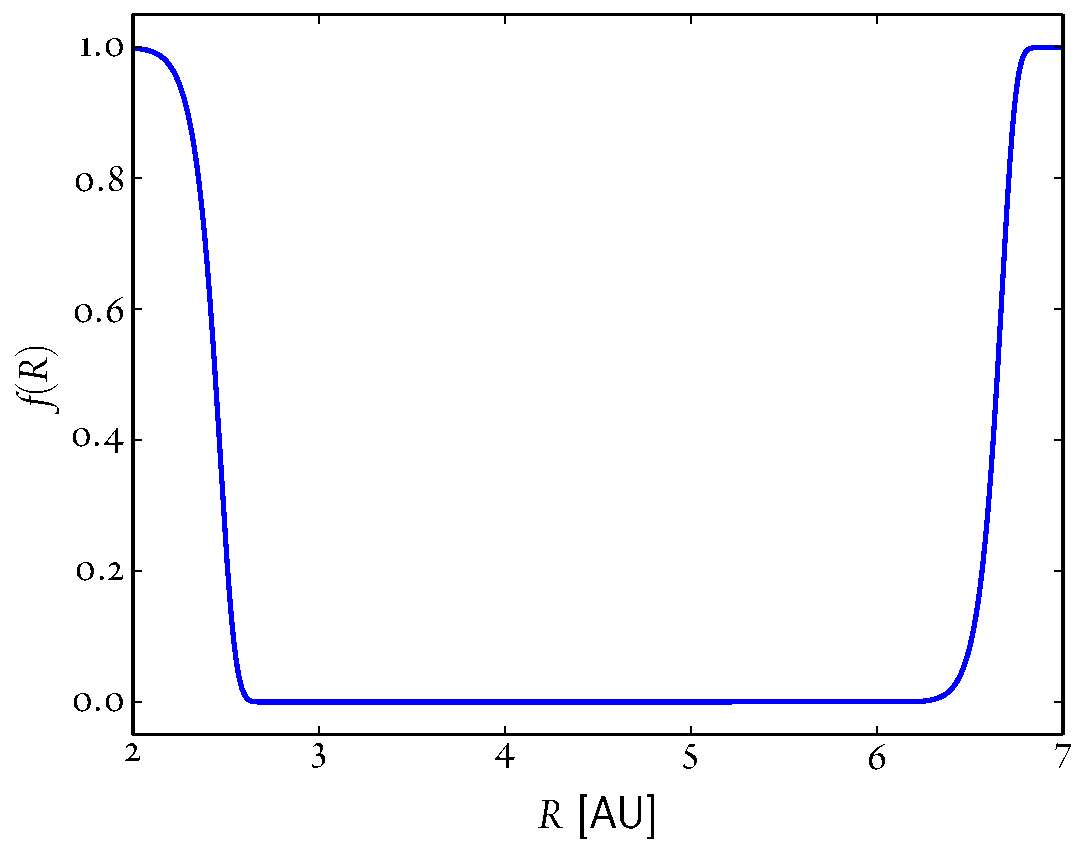
\includegraphics[width=0.5\textwidth]{figures/overlap}
   \caption{Przebieg funkcji $f(R)$ opisywanej równaniem~\mref{eq:overlap} dla
   zakresu promieni użytego we wszystkich symulacjach przedstawionych w~tej
pracy.}
   \label{fig:overlap}
\end{figure}
%
\subsection{Parametry symulacji}\label{ch2:simpar}
%
W~ramach pracy doktorskiej przeprowadzono szereg symulacji 2D modyfikując
początkowy $\epsilon$ oraz promień cząstek $a$, w~celu weryfikacji użytych metod
i wskazania optymalnych parametrów dla pełnych symulacji trójwymiarowych. Aby
móc porównać wyniki z~pracą innych autorów~\citep{JY07} parametr $\epsilon$
wybrano z~przedziału $[0.2, 2.0]$. Taki dobór parametru $\epsilon$ pozwala także
wzbudzić morfologicznie odmienny wyniki niestabilności strumieniowej, które
zostaną opisane w~dalszej części pracy. Promień cząstek pyłu został dobrany, tak
aby otrzymane wyniki można było porównać z~pracą JY, a także tak, aby były na
tyle małe aby ich obecność w~dysku protoplanetarnym można było wyjaśnić w~ramach
modelu zderzeniowego wzrostu przedstawionego w~rozdziale 1. Pełne zestawienie
użytych parametrów zostało przedstawione w~tabeli~\ref{tab1}.

\begin{table}
   \centering
   \begin{tabular}{cccccc}
      \hline
      Nazwa & $N_r \times N_\varphi \times N_z$ &
      $a$~[cm] & $\epsilon$ & $T_\textrm{end}$~[yr] \\
      \hline
      BD3d  &  $2560  \times 512 \times 192$  & 50  & 3.0 & 500  \\
      BD3dS &  $2560  \times 512 \times 192$  & 50  & 3.0 & 250  \\
      AA    &  $5120  \times 1   \times 300$  & 10  & 0.2 & 3000 \\
      AB    &  $5120  \times 1   \times 300$  & 10  & 1.0 & 3000 \\
      AC    &  $5120  \times 1   \times 300$  & 10  & 2.0 & 3000 \\
      BA    &  $5120  \times 1   \times 300$  & 50  & 0.2 & 3000 \\
      BB    &  $5120  \times 1   \times 300$  & 50  & 1.0 & 3000 \\
      BB3d  &  $2560  \times 512 \times 192$  & 50  & 1.0 & 500  \\
      BC    &  $5120  \times 1   \times 300$  & 50  & 2.0 & 3000 \\
      AAh   &  $10240 \times 1   \times 600$  & 10  & 0.2 & 1700 \\
      AAu   &  $20480 \times 1   \times 1200$ & 10  & 0.2 & 1800 \\
      ABh   &  $10240 \times 1   \times 600$  & 10  & 1.0 & 1400 \\
      BAh   &  $10240 \times 1   \times 600$  & 50  & 0.2 & 1730 \\
      BBh   &  $10240 \times 1   \times 600$  & 50  & 1.0 & 3000 \\
      \hline
   \end{tabular}
\caption{Parametry użyte w~symulacjach. Kolumny opisują w~kolejności: oznaczenie
   kodowe symulacji, ilość komórek obliczeniowych w~kierunkach $r$, $\varphi$ i
   $z$, promień cząstek, początkowy stosunek gęstości pyłu do gęstości gazu,
całkowity czas trwania symulacji w~latach.}
\label{tab1}
\end{table}

%%%%%%%%%%%%%%%%%%%%%%%%%%%%%%%%%%%%%%%%%%%%%%%%%%%%%%%%%%%%%%%%%%%%%%%%%%%%%%%%
% vim: tw=80 ts=3: 
